%============================================================
% MTH 112 Project - Inverse Trig
% Updated 202504
%============================================================

\section{Inverse Trigonometry} \label{section-inverse-trig}
In this section, we will use the inverse sine, cosine, and tangent functions, find the exact value of expressions involving the inverse-trigonometric functions, use a calculator to evaluate inverse-trigonometric functions, and find exact values of composite functions with inverse-trigonometric functions.

\textbook{\href{https://openstax.org/books/algebra-and-trigonometry-2e/pages/8-3-inverse-trigonometric-functions}{8.3}}

\subsection*{Preparation Exercises} \label{preparation-exercises-section-inverse-trig}

Answer the following without using a calculator. These questions are intended to check the prerequisite skills needed to complete the rest of the lab.

% \begin{myPrep}
% 	\begin{enumerate}
% 		\item What is the domain of\ldots
% 			\begin{enumerate}
% 				\begin{multicols}{3}
% 					\item $y=\sin(x)$
% 					\item $y=\cos(x)$
% 					\item $y=\tan(x)$
% 				\end{multicols}
% 			\end{enumerate}
% 			\vfill
% 		\item What is the range of\ldots
% 			\begin{enumerate}
% 				\begin{multicols}{3}
% 					\item $y=\sin(x)$
% 					\item $y=\cos(x)$
% 					\item $y=\tan(x)$
% 				\end{multicols}
% 			\end{enumerate}
% 			\vfill
% 	\end{enumerate}
% \end{myPrep}

% \begin{myPrep}
	% \item If $f$ is an invertible function, and the domain of $f$ is $(-2,7]$ and the range of $f$ is $(-\infty,\infty)$, what will the domain and range of $f^{-1}$ be?
	% \vfill
% \end{myPrep}

\begin{myPrep}
	\begin{multicols}{2}\raggedcolumns
		Fill in the blanks referring to the angles in Figure \ref{fig:unit-circle-coterminal-fourth-quadrant}.
		\begin{enumerate}[itemsep=1cm]
			\item $\frac{11\pi}{6}$ is coterminal with the negative angle \hrulefill.
			\item $\frac{7\pi}{4}$ is coterminal with the negative angle \hrulefill.
			\item $\frac{5\pi}{3}$ is coterminal with the negative angle \hrulefill.
			\item $\frac{3\pi}{2}$ is coterminal with the negative angle \hrulefill.
		\end{enumerate}
		\columnbreak
		\begin{center}
			\captionsetup{type=figure} \captionof{figure}{Unit Circle with Standard Values}
			\begin{tikzpicture}
				\begin{axis}[
						height=7cm,
						width=7cm,
						xmin=-.3,xmax=1.1,
						ymin=-1.1,ymax=0.3,
			       		xtick={-1},
			       		ytick={-1},
			       		% clip=false,
						]
          				\draw   (axis cs:0,0) circle [radius=1];

          				\draw   [color=fifth,thick](0,0)--(0,-1);
          				\addplot[mark=*,color=fifth] coordinates{(0,-1)} node[above left,rotate=-90] {\footnotesize$\theta=\frac{3\pi}{2}$};
          				\addplot[opacity=0.3,thin,variable=\t, domain=0:270, samples=50, color=fifth,-{latex}]({0.05*cos(t)}, {0.05*sin(t)});

          				\draw   [color=fourth,opacity=0.3](0,0)--(0.5,-0.866);
          				\addplot[mark=*,color=fourth] coordinates{(0.5,-0.866)} node[left,rotate=-60] {\footnotesize$\theta=\frac{5\pi}{3}$};
          				\addplot[opacity=0.3,thin,variable=\t, domain=0:300, samples=50, color=fourth,-{latex}]({0.1*cos(t)}, {0.1*sin(t)});

          				\draw   [color=third,opacity=0.3](0,0)--(0.707,-0.707);
          				\addplot[mark=*,color=third] coordinates{(0.707,-0.707)} node[left,rotate=-45] {\footnotesize$\theta=\frac{7\pi}{4}$};
          				\addplot[opacity=0.3,thin,variable=\t, domain=0:315, samples=50, color=third,-{latex}]({0.15*cos(t)}, {0.15*sin(t)});

          				\draw   [color=second,opacity=0.3](0,0)--(0.866,-0.5);
          				\addplot[mark=*,color=second] coordinates{(0.866,-0.5)} node[left,rotate=-30] {\footnotesize$\theta=\frac{11\pi}{6}$};
          				\addplot[opacity=0.3,thin,variable=\t, domain=0:330, samples=50, color=second,-{latex}]({0.2*cos(t)}, {0.2*sin(t)});
				\end{axis}
			\end{tikzpicture}
			\label{fig:unit-circle-coterminal-fourth-quadrant}
		\end{center}
	\end{multicols}
\end{myPrep}

\begin{myPrep}
	\begin{multicols}{2}
	The invertible function $g$ is defined by Table \ref{table:inverse-function-table}. Fill in the $g^{-1}(x)$ row. Some entries may be \say{undefined}.
	\columnbreak
			\begin{center}\captionsetup{type=table}\captionof{table}{The invertible function $g$}\label{table:inverse-function-table}
			\renewcommand{\arraystretch}{1} 
				\begin{tabular}{|| c | P{.6cm} | P{.6cm} | P{.6cm} | P{.6cm} | P{.6cm} | P{.6cm} | P{.6cm} | P{.6cm} ||}
					\hline
					$x$    & $-4$ & $-1$ & $1$ & $3$ & $6$ & $10$ & $11$\\
					\hline
					$g(x)$ & $10$ & $3$ & $6$ & $-4$ & $9$ & $-1$ & $1$\\ 
					\hline
					$g^{-1}(x)$ & & & & & & &\\ 
					\hline
				\end{tabular}
			\end{center}
	\end{multicols}
\end{myPrep}

\begin{myPrep}
	\begin{multicols}{2}
		Show in Figure \ref{fig:inverse-function} is an invertible function $y=R(x)$.
		 Draw a sketch of $y=R^{-1}(x)$ on the same figure.
		\columnbreak
			\begin{center}\captionsetup{type=figure}\captionof{figure}{Graph of $y=R(x)$}\label{fig:inverse-function}
			   	\begin{tikzpicture}
					\begin{axis}[
						height=5cm,
						width=5cm,
						framed,
						xmin=-6,xmax=6,
						ymin=-6,ymax=6,
						xtick={-4,-2,2,4},
						minor xtick={-5,-3,-1,1,3,5},
						ytick={-4,-2,2,4},
						minor ytick={-5,-3,-1,1,3,5},
						grid=both,
						]
						\addplot[color=first]coordinates{(-5,2)(-3,1)(-2,-2)};
						\addplot[color=first]coordinates{(-2,-5)(1,-4)(4,-2)};
						\addplot[only marks,color=first] coordinates{(-5,2)(-2,-5)(4,-2)};
						\addplot[only marks,color=first,fill=white] coordinates{(-2,-2)};
					\end{axis}
				\end{tikzpicture}
			\end{center}
	\end{multicols}
\end{myPrep}

%======================================================
\newpage
%======================================================

\subsection*{Practice Exercises} \label{practice-exercises-section-inverse-trig}


\begin{myPractice}
	Evaluate the expressions using your memorized values on the unit circle. Some might be undefined.
	\begin{enumerate}
		\begin{multicols}{5}
			\item $\sin^{-1}\left(\frac{1}{2}\right)$
			\item $\sin^{-1}\left(-\frac{\sqrt{3}}{2}\right)$
			\item $\cos^{-1}\left(1\right)$
			\item $\cos^{-1}\left(\pi\right)$
			\item $\cos^{-1}\left(-\frac{1}{2}\right)$
		\end{multicols}
	\end{enumerate}
\end{myPractice}
\vfill

\begin{myPractice}
	Fill in the table values using your memorized values on the unit circle.
	\begin{center}
			\renewcommand{\arraystretch}{1.5} 
				\begin{tabular}{|| c | P{1cm} | P{1cm} | P{1cm} | P{1cm} | P{1cm} | P{1cm} | P{1cm} | P{1cm} | P{1cm} | P{1cm} ||}
					\hline
					$t$    & $1$ & $\frac{\sqrt{3}}{2}$ & $\frac{\sqrt{2}}{2}$ & $\frac{1}{2}$ & $0$ & $-\frac{1}{2}$ & $-\frac{\sqrt{2}}{2}$ & $-\frac{\sqrt{3}}{2}$ & $-1$\\
					\hline
					$\cos^{-1}(t)$ & & & & & & & & &\\ 
					\hline
					$\sin^{-1}(t)$ & & & & & & & & &\\ 
					\hline
				\end{tabular}
			\end{center}
\end{myPractice}

\begin{myPractice}
	\begin{multicols}{2}
		Fill in the table below with standard values of inverse trigonometric functions without a calculator. If the value of $z$ is blank, start by filling that in first.
		\columnbreak
		\begin{center}
		\renewcommand{\arraystretch}{1.5} 
			\begin{tabular}{|| c | c | c | c ||}
				\hline
				$z$    					& $\sin^{-1}(z)$ 	& $\cos^{-1}(z)$ 		& $\tan^{-1}(z)$ \\
				\hline
				$0$ 					& 	 				& 				 		& \\
				\hline
										& $-\frac{\pi}{2}$ 	& 		 				& \\
				\hline
										& 				 	& $\frac{\pi}{6}$ 		& N/A \\
				\hline
										& 				 	& 	 					& $\frac{\pi}{4}$ \\
				\hline
				$\frac{\sqrt{2}}{2}$ 	& 				 	& 				 		& N/A \\
				\hline
							 			& 				 	& $\frac{2\pi}{3}$ 		& N/A \\
				\hline
			\end{tabular}
		\end{center}
	\end{multicols}
\end{myPractice}

\begin{myPractice}
	Use a calculator to approximate the values below.
	\begin{enumerate}
		\begin{multicols}{5}
			\item $\sin^{-1}(0.1)$
			\vfill
			\item $\cos^{-1}(0.6)$
			\vfill
			\item $\tan^{-1}(2)$
			\vfill
			\item $\sec^{-1}(-2)$
			\vfill
			\item $\csc^{-1}(3)$
			\vfill
		\end{multicols}
	\end{enumerate}
\end{myPractice}
\vfill

%======================================================
\newpage
%======================================================

\begin{myPractice}
Use inverse trigonometry to find the missing angles.
	\begin{enumerate}
		\begin{multicols}{2}
			\item Use inverse trigonometry and a calculator to find the missing angles $\alpha$ and $\beta$ in the triangle shown in Figure \ref{fig:section-inverse-trig-example-triangle}.
			 Drawing not to scale.
			\columnbreak
			\begin{center}\captionsetup{type=figure} \captionof{figure}{A right triangle}
				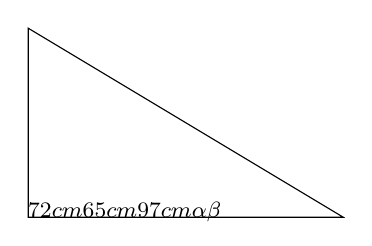
\begin{tikzpicture}[thin] \label{fig:section-inverse-trig-example-triangle}
					\coordinate (O) at (0,0);
					\coordinate (A) at (4,0);
					\coordinate (B) at (0,12/5);
					\draw (O)--(A)--(B)--cycle;
					\footnotesize
					\tkzLabelSegment[below=2pt](O,A){$72\text{cm}$}
					\tkzLabelSegment[above=2pt,rotate=90](O,B){$65\text{cm}$}
					\tkzLabelSegment[above=2pt, rotate=-atan(2/3)](A,B){$97\text{cm}$}
					\tkzMarkRightAngle[size=0.5](A,O,B)
					\tkzMarkAngle[size=0.8cm](B,A,O)
					\tkzLabelAngle[pos = 0.6](B,A,O){$\alpha$}
					\tkzMarkAngle[size=0.7cm](O,B,A)
					\tkzLabelAngle[pos = 0.5](O,B,A){$\beta$}
				\end{tikzpicture}
			\end{center}
		\end{multicols}
		\vfill

		\begin{multicols}{2}
			\item Imagine designing a birdhouse to make out of wood. The sides of this birdhouse are shaped like trapezoids, with dimensions shown in Figure \ref{fig:section-inverse-trig-birdhouse}. Find the angle $\phi$, in degrees, using inverse trigonometry and your calculator. Note: this angle will be related to how you set up your saw to cut the wood correctly.
			\columnbreak
			\begin{center}\captionsetup{type=figure} \captionof{figure}{The side of a birdhouse}
				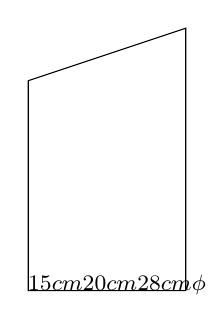
\begin{tikzpicture}[thin] \label{fig:section-inverse-trig-birdhouse}
					\coordinate (O) at (0,0);
					\coordinate (A) at (2,0);
					\coordinate (B) at (2,10/3);
					\coordinate (C) at (0,8/3);
					\draw (O)--(A)--(B)--(C)--cycle;
					\footnotesize
					\tkzLabelSegment[below=2pt](O,A){$15\text{cm}$}
					\tkzLabelSegment[above=2pt,rotate=90](O,C){$20\text{cm}$}
					\tkzLabelSegment[below=2pt,rotate=90](A,B){$28\text{cm}$}
					\tkzMarkRightAngle[size=0.5](C,O,A)
					\tkzMarkAngle[size=0.7cm](C,B,A)
					\tkzLabelAngle[pos = 0.5](C,B,A){$\phi$}
				\end{tikzpicture}
			\end{center}
		\end{multicols}
	\end{enumerate}
\end{myPractice}
\vfill

\begin{myPractice}
Evaluate the following expressions without a calculator.
	\begin{enumerate}
		\begin{multicols}{2}
			% \item $\cos^{-1}\left(\cos\left(\frac{\pi}{3}\right)\right)$
			\item $\cos^{-1}\left(\cos\left(\frac{2\pi}{3}\right)\right)$
			\vspace{3cm}
			\item $\cos^{-1}\left(\cos\left(-\frac{\pi}{3}\right)\right)$
			\columnbreak
			\item $\cos^{-1}\left(\cos\left(\frac{4\pi}{3}\right)\right)$
			\vspace{3cm}
			% \item $\cos^{-1}\left(\cos\left(\frac{\pi}{7}\right)\right)$
			\item $\cos^{-1}\left(\cos\left(\frac{6\pi}{7}\right)\right)$
			% \item $\cos^{-1}\left(\cos\left(-\frac{2\pi}{7}\right)\right)$
			% \item $\cos^{-1}\left(\cos\left(\frac{9\pi}{7}\right)\right)$
		\end{multicols}
	\end{enumerate}
\end{myPractice}
\vspace{3cm}

%======================================================
\newpage
%======================================================

\begin{myPractice}
Evaluate the following expressions without a calculator.
	\begin{enumerate}
		\begin{multicols}{2}
			\item $\sin\left(\cos^{-1}\left(\frac{2}{3}\right)\right)$
			\vspace{4cm}
			\item $\sin\left(\tan^{-1}\left(\frac{4}{7}\right)\right)$
			\item $\cos\left(\sin^{-1}\left(-\frac{1}{5}\right)\right)$
			\vspace{4cm}
			\item $\cos\left(\tan^{-1}\left(-\frac{7}{2}\right)\right)$
		\end{multicols}
	\end{enumerate}
\end{myPractice}
\vspace{4cm}

% \begin{myPractice}
% 	\begin{multicols}{2}
% 		Find the formula for the inverse function of the function $f(x)=4\sin\left(\frac{\pi}{6}(x-1)\right)+2$ on the domain $[-2,4]$. Both the graph of $f$ and $f^{-1}$ are shown in Figure \ref{fig:section-inverse-trig-inverse-of-sine}. Note that they are reflections of each other over the line $y=x$.
% 		\columnbreak

% 		\begin{center}\captionsetup{type=figure} \captionof{figure}{A graph of $f$ and $f^{-1}$}
% 			\begin{tikzpicture} \label{fig:section-inverse-trig-inverse-of-sine}
% 	 			\begin{axis}[
% 	 				framed,
% 	 				xmin=-3,xmax=7,
% 	 				ymin=-3,ymax=7,
% 				    xtick={-2,-1,...,6},
% 				    ytick={-2,-1,...,6},
% 				    grid=both,
% 	 				]
% 					\addplot[first,line width=1.5pt,samples=100]expression[domain=-2:4]{4*sin(30*(x-1))+2};
% 					\addplot[first,mark=*,only marks]coordinates{(-2,-2) (4,6)};
% 					\addplot[second,line width=1.5pt,samples=100,dashdotted]expression[domain=-2:6]{1/30*asin((x-2)/4)+1};
% 					\addplot[second,mark=*,only marks]coordinates{(-2,-2) (6,4)};
% 					\addplot[third,line width=1pt,samples=100,dashed]expression[domain=-3:7]{x};
% 	 			\end{axis}
% 			\end{tikzpicture}
% 		\end{center}
% 	\end{multicols}
% \end{myPractice}

\begin{myPractice}
In this exercise, discuss some of the details about inverse trigonometry with your group members.
	\begin{enumerate}
		\item What are the similarities and differences between $\sin^{-1}(x)$ and $\csc(x)$? Start by discussing the meaning of the inputs and outputs of the functions.
		\vfill
		\item What are the similarities and differences between $\sin^{-1}(x)$ and $\sin^2(x)$? Start by discussing the meaning of the inputs and outputs of the functions.
		\vfill
		\item The range of both $\sin^{-1}(x)$ and $\tan^{-1}(x)$ is in quadrants I and IV. The range of $\cos^{-1}(x)$ is in quadrants I and II. Why do you think that none of the inverse trigonometric functions use quadrant III?
		\vfill
		\item If Georgiana said that, \say{I think that the value of $\sin^{-1}(-1)$ is $\frac{3\pi}{2}$,} how would you help her understand her mistake?
		\vfill
	\end{enumerate}
\end{myPractice}

%======================================================
\newpage
%======================================================

\subsection*{Definitions} \label{definitions-section-inverse-trig}

\begin{multicols}{2}
	\begin{myDefinition}[{Inverse cosine}]~\\[0.5mm]
		The \textbf{inverse cosine function} inputs a $x$-value on the unit circle and outputs the angle from $0$ to $\pi$ that matches that $x$-value, as shown in Figure \ref{fig:Unit-circle-inverse-cos-values}. Another way to say that is that for angles, $\theta$, in the interval $\left[0,\pi\right]$, if $\cos(\theta)=x$ then $\cos^{-1}(x)=\theta$.
		\begin{center}\captionsetup{type=table}\captionof{table}{Domain and range for cosine and cosine inverse}\label{table:section-inverse-trig-definition-cosine-inverse}
			\renewcommand{\arraystretch}{1.5}
			\begin{tabular}{|| p{2.3cm} | p{2.3cm} | p{2.3cm} ||}
				\hline
				Function			& $\cos(z)$										& $\cos^{-1}(z)$									\\
				\hline
				Domain and meaning	& $\mathbb{R}$\newline Angles on unit circle	& $[-1,1]$\newline $x$-values on unit circle		\\
				\hline
				Range and meaning	& $[-1,1]$\newline $x$-values on unit circle	& $\left[0,\pi\right]$\newline Angles on unit circle	\\
				\hline
			\end{tabular}
		\end{center}
		\columnbreak
		\begin{center}
			\captionsetup{type=figure}\captionof{figure}{Unit Circle with Standard Inverse Cosine Values}
			\begin{tikzpicture}
				\begin{axis}[
						height=5cm,
						width=5cm,
						xmin=-1,xmax=1,
						ymin=-1,ymax=1,
			       		xtick={-1,1},
			       		ytick={-1,1},
			       		clip=false,
						]
						\draw 	(axis cs:0,0) circle [radius=1];

						\addplot[mark=*,color=first] coordinates{(1,0)} 
						node[right] {\footnotesize$\cos^{-1}\left(1\right)=0$};

						\addplot[mark=*,color=first] coordinates{(-1,0)} 
						node[left] {\footnotesize$\cos^{-1}\left(-1\right)=\pi$};

						\draw   [color=second,opacity=0.3](0,0)--(0.866,0.5);
						\addplot[mark=*,color=second] coordinates{(0.866,0.5)} 
						node[right,rotate=30] {\footnotesize$\cos^{-1}\left(\frac{\sqrt3}{2}\right)=\frac{\pi}{6}$};

						\draw   [color=third,opacity=0.3](0,0)--(0.707,0.707);
						\addplot[mark=*,color=third] coordinates{(0.707,0.707)}
						node[right,rotate=45] {\footnotesize$\cos^{-1}\left(\frac{\sqrt2}{2}\right)=\frac{\pi}{4}$};

						\draw   [color=fourth,opacity=0.3](0,0)--(0.5,0.866);
						\addplot[mark=*,color=fourth] coordinates{(0.5,0.866)}
						node[right,rotate=60] {\footnotesize$\cos^{-1}\left(\frac{1}{2}\right)=\frac{\pi}{3}$};

						\draw   [color=fourth,opacity=0.3](0,0)--(0,1);
						\addplot[mark=*,color=fifth] coordinates{(0,1)}
						node[right,rotate=90] {\footnotesize$\cos^{-1}\left(0\right)=\frac{\pi}{2}$};

						\draw   [color=fourth,opacity=0.3](0,0)--(-0.5,0.866);
						\addplot[mark=*,color=fourth] coordinates{(-0.5,0.866)}
						node[left,rotate=-60] {\footnotesize$\cos^{-1}\left(-\frac{1}{2}\right)=\frac{2\pi}{3}$};

						\draw   [color=third,opacity=0.3](0,0)--(-0.707,0.707);
						\addplot[mark=*,color=third] coordinates{(-0.707,0.707)}
						node[left,rotate=-45] {\footnotesize$\cos^{-1}\left(-\frac{\sqrt2}{2}\right)=\frac{3\pi}{4}$};

						\draw   [color=second,opacity=0.3](0,0)--(-0.866,0.5);
						\addplot[mark=*,color=second] coordinates{(-0.866,0.5)}
						node[left,rotate=-30] {\footnotesize$\cos^{-1}\left(-\frac{\sqrt3}{2}\right)=\frac{5\pi}{6}$};

						\addplot[name path=f,domain=-1:1,thick,color=first,samples=100] {(1-x^2)^(0.5)};
    					\path[name path=axis,ultra thin] (axis cs:-1,0) -- (axis cs:1,0);
    					\addplot [thick,color=first,fill=first,fill opacity=0.1] fill between[of=f and axis,soft clip={domain=-1:1}];
				\end{axis}
			\end{tikzpicture}
			\label{fig:Unit-circle-inverse-cos-values}
		\end{center}
	\end{myDefinition}
\end{multicols}

\begin{multicols}{2}
	\begin{myDefinition}[{Inverse sine}]~\\[0.5mm]
		The \textbf{inverse sine function} inputs a $y$-value on the unit circle and outputs the angle from $-\frac{\pi}{2}$ to $\frac{\pi}{2}$ that matches that $y$-value, as shown in Figure \ref{fig:Unit-circle-inverse-sin-values}. Another way to say that is that for angles, $\theta$, in the interval $\left[-\frac{\pi}{2},\frac{\pi}{2}\right]$, if $\sin(\theta)=y$ then $\sin^{-1}(y)=\theta$.
		\begin{center}\captionsetup{type=table}\captionof{table}{Domain and range for sine and sine inverse}\label{table:section-inverse-trig-definition-sine-inverse}
			\renewcommand{\arraystretch}{1.5}
			\begin{tabular}{|| p{2.3cm} | p{2.3cm} | p{2.3cm} ||}
				\hline
				Function			& $\sin(z)$										& $\sin^{-1}(z)$								\\
				\hline
				Domain and meaning	& $\mathbb{R}$\newline Angles on unit circle	& $[-1,1]$\newline $y$-values on unit circle	\\
				\hline
				Range and meaning	& $[-1,1]$\newline $y$-values on unit circle	& $\left[-\frac{\pi}{2},\frac{\pi}{2}\right]$\newline Angles on unit circle\\
				\hline
			\end{tabular}
		\end{center}
		\columnbreak
		\begin{center}
			\captionsetup{type=figure} \captionof{figure}{Unit Circle with Standard Inverse Sine Values}
			\begin{tikzpicture}
				\begin{axis}[
						height=5cm,
						width=5cm,
						xmin=-1,xmax=1,
						ymin=-1,ymax=1,
			       		xtick={-1,1},
			       		ytick={-1,1},
			       		clip=false,
						]
						\draw 	(axis cs:0,0) circle [radius=1];
						\addplot[mark=*,color=first] coordinates{(1,0)} 
						node[right] {\footnotesize$\sin^{-1}(0)=0$};

						\addplot[mark=*,color=fifth] coordinates{(0,1)} 
						node[right,rotate=90] {\footnotesize$\sin^{-1}\left(1\right)=\frac{\pi}{2}$};

						\draw   [color=fourth,opacity=0.3](0,0)--(0.5,0.866);
						\addplot[mark=*,color=fourth] coordinates{(0.5,0.866)} 
						node[right,rotate=60] {\footnotesize$\sin^{-1}\left(\frac{\sqrt3}{2}\right)=\frac{\pi}{3}$};

						\draw   [color=third,opacity=0.3](0,0)--(0.707,0.707);
						\addplot[mark=*,color=third] coordinates{(0.707,0.707)} 
						node[right,rotate=45] {\footnotesize$\sin^{-1}\left(\frac{\sqrt2}{2}\right)=\frac{\pi}{4}$};

						\draw   [color=second,opacity=0.3](0,0)--(0.866,0.5);
						\addplot[mark=*,color=second] coordinates{(0.866,0.5)} 
						node[right,rotate=30] {\footnotesize$\sin^{-1}\left(\frac{1}{2}\right)=\frac{\pi}{6}$};

						\addplot[mark=*,color=first] coordinates{(1,0)} 
						node[right] {\footnotesize$\sin^{-1}(0)=0$};

						\draw   [color=second,opacity=0.3](0,0)--(0.866,-0.5);
						\addplot[mark=*,color=second] coordinates{(0.866,-0.5)} 
						node[right,rotate=-30] {\footnotesize$\sin^{-1}\left(-\frac{1}{2}\right)=-\frac{\pi}{6}$};

						\draw   [color=third,opacity=0.3](0,0)--(0.707,-0.707);
						\addplot[mark=*,color=third] coordinates{(0.707,-0.707)} 
						node[right,rotate=-45] {\footnotesize$\sin^{-1}\left(-\frac{\sqrt2}{2}\right)=-\frac{\pi}{4}$};

						\draw   [color=fourth,opacity=0.3](0,0)--(0.5,-0.866);
						\addplot[mark=*,color=fourth] coordinates{(0.5,-0.866)} 
						node[right,rotate=-60] {\footnotesize$\sin^{-1}\left(-\frac{\sqrt3}{2}\right)=-\frac{\pi}{3}$};

						\addplot[mark=*,color=fifth] coordinates{(0,-1)} 
						node[right,rotate=-90] {\footnotesize$\sin^{-1}\left(-1\right)=-\frac{\pi}{2}$};

						\addplot[name path=f,domain=0:1,thick,color=first,samples=100] {(1-x^2)^(0.5)};
    					\path[name path=axis,ultra thin] (axis cs:0,0) -- (axis cs:1,0);
    					\addplot [thick,color=first,fill=first,fill opacity=0.1] fill between[of=f and axis,soft clip={domain=0:1}];

    					\addplot[name path=g,domain=0:1,thick,color=first,samples=100] {-(1-x^2)^(0.5)};
    					\addplot [thick,color=first,fill=first,fill opacity=0.1] fill between[of=g and axis,soft clip={domain=0:1}];
				\end{axis}
			\end{tikzpicture}
			\label{fig:Unit-circle-inverse-sin-values}
		\end{center}
	\end{myDefinition}
\end{multicols}

%======================================================
\newpage
%======================================================

\begin{multicols}{2}
	\begin{myDefinition}[{Inverse tangent}]~\\[0.5mm]
		The \textbf{inverse tangent function} inputs a slope, $m$, and outputs the angle from $-\frac{\pi}{2}$ to $\frac{\pi}{2}$ (non-inclusive) that matches that slope, as shown in Figure \ref{fig:Unit-circle-inverse-tan-values}. Another way to say that is that for angles, $\theta$, in the interval $\left(-\frac{\pi}{2},\frac{\pi}{2}\right)$, if $\tan(\theta)=m$ then $\tan^{-1}(m)=\theta$.
		\begin{center}\captionsetup{type=table}\captionof{table}{Domain and range for sine and sine inverse}\label{table:section-inverse-trig-definition-tan-inverse}
			\renewcommand{\arraystretch}{1.5}
			\begin{tabular}{|| p{2.3cm} | p{2.4cm} | p{2.3cm} ||}
				\hline
				Function			& $\tan(z)$										& $\tan^{-1}(z)$								\\
				\hline
				Domain and meaning	& $\mathbb{R}$ except odd multiples of $\frac{\pi}{2}$\newline Angles on unit circle	& $\mathbb{R}$\newline Slopes		\\
				\hline
				Range and meaning	& $\mathbb{R}$\newline Slopes		& $\left(-\frac{\pi}{2},\frac{\pi}{2}\right)$\newline Angles on unit circle\\
				\hline
			\end{tabular}
		\end{center}
		\columnbreak
		\begin{center}
			\captionsetup{type=figure} \captionof{figure}{Unit Circle with Standard Inverse Tangent Values}
			\begin{tikzpicture}
				\begin{axis}[
						height=5cm,
						width=5cm,
						xmin=-1,xmax=1,
						ymin=-1,ymax=1,
			       		xtick={-1,1},
			       		ytick={-1,1},
			       		clip=false,
						]
						\draw 	(axis cs:0,0) circle [radius=1];

						\addplot[mark=*,color=first] coordinates{(1,0)} 
						node[right] {\footnotesize$\tan^{-1}(0)=0$};

						\draw   [color=fourth,opacity=0.3](0,0)--(0.5,0.866);
						\addplot[mark=*,color=fourth] coordinates{(0.5,0.866)} 
						node[right,rotate=60] {\footnotesize$\tan^{-1}\left(\sqrt3\right)=\frac{\pi}{3}$};

						\draw   [color=third,opacity=0.3](0,0)--(0.707,0.707);
						\addplot[mark=*,color=third] coordinates{(0.707,0.707)} 
						node[right,rotate=45] {\footnotesize$\tan^{-1}\left(1\right)=\frac{\pi}{4}$};

						\draw   [color=second,opacity=0.3](0,0)--(0.866,0.5);
						\addplot[mark=*,color=second] coordinates{(0.866,0.5)} 
						node[right,rotate=30] {\footnotesize$\tan^{-1}\left(\frac{\sqrt3}{3}\right)=\frac{\pi}{6}$};

						\addplot[mark=*,color=first] coordinates{(1,0)} 
						node[right] {\footnotesize$\tan^{-1}(0)=0$};

						\draw   [color=second,opacity=0.3](0,0)--(0.866,-0.5);
						\addplot[mark=*,color=second] coordinates{(0.866,-0.5)} 
						node[right,rotate=-30] {\footnotesize$\tan^{-1}\left(-\frac{\sqrt3}{3}\right)=-\frac{\pi}{6}$};

						\draw   [color=third,opacity=0.3](0,0)--(0.707,-0.707);
						\addplot[mark=*,color=third] coordinates{(0.707,-0.707)} 
						node[right,rotate=-45] {\footnotesize$\tan^{-1}\left(-1\right)=-\frac{\pi}{4}$};

						\draw   [color=fourth,opacity=0.3](0,0)--(0.5,-0.866);
						\addplot[mark=*,color=fourth] coordinates{(0.5,-0.866)} 
						node[right,rotate=-60] {\footnotesize$\tan^{-1}\left(-\sqrt3\right)=-\frac{\pi}{3}$};

						\addplot[name path=f,domain=0:1,thick,color=first,samples=100] {(1-x^2)^(0.5)};
    					\path[name path=axis,ultra thin] (axis cs:0,0) -- (axis cs:1,0);
    					\addplot [thick,color=first,fill=first,fill opacity=0.1] fill between[of=f and axis,soft clip={domain=0:1}];

    					\addplot[name path=g,domain=0:1,thick,color=first,samples=100] {-(1-x^2)^(0.5)};
    					\addplot [thick,color=first,fill=first,fill opacity=0.1] fill between[of=g and axis,soft clip={domain=0:1}];

    					\addplot[mark=*,color=fifth,fill=white] coordinates{(0,1)};
						\addplot[mark=*,color=fifth,fill=white] coordinates{(0,-1)};
				\end{axis}
			\end{tikzpicture}
			\label{fig:Unit-circle-inverse-tan-values}
		\end{center}
	\end{myDefinition}
\end{multicols}

%======================================================
\newpage
%======================================================

\subsection*{Exit Exercises} \label{exit-exercises-section-inverse-trig}

\begin{myExit}
	Fill in the blanks to show how should you think about the inputs and outputs of each function? The answer to each is either \say{an angle}, \say{an $x$-value on the unit circle}, or \say{a $y$-value on the unit circle}.
		\begin{enumerate}[itemsep=0.5cm]
			\item $\text{\underline{\phantom{your answer your answer your answer}}} =\sin\left(\text{\underline{\phantom{your answer your answer your answer}}}\right)$.
			\item $\text{\underline{\phantom{your answer your answer your answer}}} =\cos\left(\text{\underline{\phantom{your answer your answer your answer}}}\right)$.
			\item $\text{\underline{\phantom{your answer your answer your answer}}} =\sin^{-1}\left(\text{\underline{\phantom{your answer your answer your answer}}}\right)$.
			\item $\text{\underline{\phantom{your answer your answer your answer}}} =\cos^{-1}\left(\text{\underline{\phantom{your answer your answer your answer}}}\right)$.
		\end{enumerate}
\end{myExit}

\begin{myExit}
	Evaluate $\cos^{-1}\left(\cos\left(\frac{5\pi}{4}\right)\right)$
\end{myExit}
\vfill
\vfill

% \begin{myExit}
		% Evaluate $\cos\left(\sin^{-1}\left(-\frac{2}{9}\right)\right)$
		% \vfill
% \end{myExit}
% \vfill
% \vfill

\begin{multicols}{2}
	\begin{myExit}
		Fill in the missing values in Table \ref{table:section-inverse-trig-exit-table}.
		\begin{center}\captionsetup{type=table}\captionof{table}{A table of inverse trigonometry}\label{table:section-inverse-trig-exit-table}
		\renewcommand{\arraystretch}{1.5} 
			\begin{tabular}{|| c | c | c ||}
				\hline
				$z$    					& $\sin^{-1}(z)$ 	& $\cos^{-1}(z)$   	\\
				\hline
										& 					& $\frac{\pi}{3}$ 	\\
				\hline
									 	& $-\frac{\pi}{4}$ 	& 				 	\\
				\hline
				$-\frac{\sqrt{3}}{2}$ 	& 				 	& 				 	\\
				\hline
			\end{tabular}
		\end{center}
	\end{myExit}

	\columnbreak

	\begin{myExit}
		Use inverse trigonometry and a calculator to find the missing angle $\zeta$ in the triangle shown in Figure \ref{fig:section-inverse-trig-exit-triangle}.
		 Drawing not to scale.
		\begin{center}\captionsetup{type=figure} \captionof{figure}{A right triangle}
			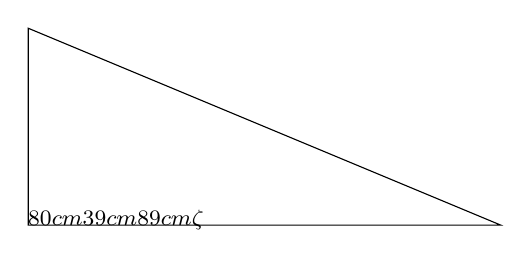
\begin{tikzpicture}[thin] \label{fig:section-inverse-trig-exit-triangle}
				\coordinate (O) at (0,0);
				\coordinate (A) at (6,0);
				\coordinate (B) at (0,2.5);
				\draw (O)--(A)--(B)--cycle;
				\footnotesize
				\tkzLabelSegment[below=2pt](O,A){$80\text{cm}$}
				\tkzLabelSegment[above=2pt,rotate=90](O,B){$39\text{cm}$}
				\tkzLabelSegment[above=2pt, rotate=-atan(5/12)](A,B){$89\text{cm}$}
				\tkzMarkRightAngle[size=0.5](A,O,B)
				\tkzMarkAngle[size=0.7cm](O,B,A)
				\tkzLabelAngle[pos = 0.5](O,B,A){$\zeta$}
			\end{tikzpicture}
		\end{center}
	\end{myExit}
\end{multicols}
\vfill
\vfill
\exitlikert{inverse trigonometry}

% \begin{center}
% 	\renewcommand{\arraystretch}{1.5} 
% 		\begin{tabular}{|| c | c | c | c ||}
% 			\hline
% 			$z$    					& $\sin^{-1}(z)$ 	& $\cos^{-1}(z)$ 		& $\tan^{-1}(z)$ \\
% 			\hline
% 			$0$ 					& $0$ 				& $\frac{\pi}{2}$ 		& $0$ \\
% 			\hline
% 			$\frac{1}{2}$ 			& $\frac{\pi}{6}$ 	& $\frac{\pi}{3}$ 		& NA \\
% 			\hline
% 			$\frac{\sqrt{2}}{2}$ 	& $\frac{\pi}{4}$ 	& $\frac{\pi}{4}$ 		& NA \\
% 			\hline
% 			$\frac{\sqrt{3}}{2}$ 	& $\frac{\pi}{3}$ 	& $\frac{\pi}{6}$ 		& NA \\
% 			\hline
% 			$1$ 					& $\frac{\pi}{2}$ 	& $0$ 					& $\frac{\pi}{4}$ \\
% 			\hline
% 			$-\frac{1}{2}$ 			& $-\frac{\pi}{6}$ 	& $\frac{2\pi}{3}$ 		& NA \\
% 			\hline
% 			$-\frac{\sqrt{2}}{2}$ 	& $-\frac{\pi}{4}$ 	& $\frac{3\pi}{4}$ 		& NA \\
% 			\hline
% 			$-\frac{\sqrt{3}}{2}$ 	& $-\frac{\pi}{3}$ 	& $\frac{5\pi}{6}$ 		& NA  \\
% 			\hline
% 			$-1$ 					& $-\frac{\pi}{2}$ 	& $\pi$ 				& $-\frac{\pi}{4}$ \\
% 			\hline
% 		\end{tabular}
% 	\end{center}